%%%%%%%%%%%%%%%%%%%%%%%%%%%%%%%%%%%%%%%%%
% Medium Length Professional CV
% LaTeX Template
% Version 2.0 (8/5/13)
%
% This template has been downloaded from:
% http://www.LaTeXTemplates.com
%
% Original author:
% Trey Hunner (http://www.treyhunner.com/)
%
% Important note:
% This template requires the resume.cls file to be in the same directory as the
% .tex file. The resume.cls file provides the resume style used for structuring the
% document.
%
%%%%%%%%%%%%%%%%%%%%%%%%%%%%%%%%%%%%%%%%%

%----------------------------------------------------------------------------------------
%	PACKAGES AND OTHER DOCUMENT CONFIGURATIONS
%----------------------------------------------------------------------------------------

\documentclass{resume} % Use the custom resume.cls style
%\usepackage{draftwatermark}
%\SetWatermarkScale{0.5}
%\SetWatermarkText{latexstudio.net}
\usepackage[left=0.4in,top=0.30in,right=0.4in,bottom=0.30in]{geometry} % Document margins
\geometry{paperheight=29.7cm}
\usepackage{paralist}
%\linespread{0.5}
\usepackage{marvosym}
\usepackage{graphicx}
\usepackage{multirow}
\usepackage{fontawesome}
\usepackage[hidelinks]{hyperref}
\usepackage[sc]{mathpazo}
%\linespread{1.05}         % Palatino needs more leading (space between lines)
\usepackage[T1]{fontenc}
\usepackage[letterspace=50]{microtype} % Single line spacing
%\usepackage{fancyhdr}
%\fancypagestyle{plain}{%
%\fancyhf{} % clear all header and footer fields
%\fancyhead[r]{\LaTeX ~StuDio $\cdot$ latexstudio@yeah.net  %$\cdot$ \thepage  
%} % except the center
%\renewcommand{\headrulewidth}{0pt}
%\renewcommand{\footrulewidth}{0pt}}
% \renewcommand{\href}{}


\name{\sc  Qian QU} % Your name
\address{
{\Large \faMapMarker} 1146 Harrison St, Seattle, WA, 98109\quad
{\Large \faMobilePhone} 434-328-0936\quad
% \quad
%\href{https://stackoverflow.com/users/5685664/jiahao}{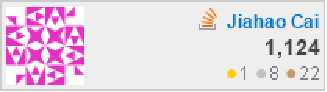
\includegraphics[width=.23\textwidth]{imgs/so.pdf}}\quad
%} % Your phone number and email
%\address {
{\Large \faEnvelopeO}  qq8jn@virginia.edu
{\Large \href{https://quq99.github.io}{\faLink}} \href{https://quq99.github.io}{quq99.github.io}\quad
{\Large\href{https://github.com/quq99}{\faGithub}} \href{https://github.com/quq99}{github.com/quq99}\quad
%{\Large\href{https://stackoverflow.com/users/5685664/jiahao}{\faStackOverflow}}
%{\href{https://stackoverflow.com/users/5685664/jiahao}{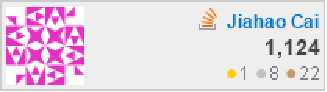
\includegraphics[trim=0 0.1cm 0 1cm, width=.23\textwidth]{imgs/so.pdf}}}
}
%\address {
% \href{https://stackoverflow.com/users/5685664/jiahao}{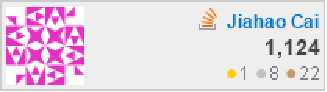
\includegraphics[width=.23\textwidth]{imgs/so.pdf}}\quad
%}

%\address{
%\faEnvelopeO \,jc4mf@virginia.edu\quad
%\faMobilePhone \,+1 434-227-3265\quad
%{\Large\href{https://people.virginia.edu/~jc4mf/}{\faHome}\quad
%\href{https://github.com/jiahao42}{\faGithub}\quad
%\href{https://stackoverflow.com/users/5685664/jiahao}{\faStackOverflow}\quad}
%} % Your phone number and email

\begin{document}

\pagestyle{empty}

%----------------------------------------------------------------------------------------
%	EDUCATION SECTION
%----------------------------------------------------------------------------------------

\begin{rSection}{\sc Education}
	\begin{Education2}
	{University of Virginia}{Charlottesville, VA, United States}{Master of Computer Science, GPA: 3.9/4.0}{Aug 2018 - Dec 2019}
	
	%\item Course: Data Structure and Algorithms, Compiler, Software Engineering, Machine Learning, Natural Language Processing(A+), Deep Learning for Visual Recognition, Statistical Learning and Graphical Models, Cloud Computing
	\end{Education2}

	\begin{Education}
		{Nanjing University}{Nanjing, China}{Master of Electronic and Communication Engineering(\textbf{postgraduate recommendation}), GPA: 4.38 / 5.0}{Sep 2015 - Jul 2018}{Bachelor of Electronic Information Science and Technology, GPA: 4.26 / 5.0, Top 15\%}{Sep 2011 - Jul 2015}
		%\item Course: Data Structure, Object-oriented programming, Java Web, Operating Systems, Mobile Development, Database
		\item Awards:  First Prize of Postgraduate Scholarship(twice), 2015\&2017
		\newline  \hphantom{Awards:} Second Prize of the People’s Scholarship, 2012
	\end{Education}

\end{rSection}

\begin{rSection}{Working Experience}

\begin{rSubsection}{\textit{Amazon.com} - Seattle, WA}{\textit{Mar 2020 -- present}}{Software Development Engineer}

\textbf{Brand Classifier(BC) onboard to Item Pipeline \textit{(Guice, IONJava, JAX-RS, AWS: S3, DynamoDB, SDK, CloudWatch, Sagemaker)}}
\item Onboarded BC Online Service as an Plugin to Item Pipeline that provides 2000TPS brand predictions to Contributions.
\item Updated ML model in service and improved the recall from 46\% to 74\% at precision 95\% for US, CA marketplace.
\item Implemented Confidence Score Normalization and Globalizer for multi-marketplace predictions.
\item Contributed to Operational Readiness including dashboard metrics, monitors, alarms and run-books.
\item Created Integration test for checking the correctness of the model predictions.

\textbf{Brand Classifier M3 model training/evaluation workflow \textit{(Guice, AWS: Lambda, S3, DynamoDB, CloudFormation, CloudWatch, EMR, Spark, SQS, Sagemaker, AMS, M3)}}
\item Created a workflow that automatically train/evaluate the ML models for ASIN/EPC/Contribution over 12 marketplace.
\item Orchestrated the workflow using AWS Lambda Functions triggered by designed M3 template.
\item Integrated Data Acquire, PreLabel, Label, PostLabel and Train/Evaluate steps and provided UI for better management. 
\item Implemented different sampling strategies for ASIN/EPC/Contribution skew data using Spark.

\textbf{Brand Classifier brand safelist Elastic Search(ES) service \textit{(AWS: API Gateway, Elastic Search, Lambda, AMS)}}
\item Utilized AWS ES to support 700K brands safelist at scale to improve tagging speed, accuracy and model performance.
\item Integrated with safelist generation workflow to automatically upload and index safelist for each brand catalog version.
\item Integrated with M3 workflow and AMS tool to automatically use the latest brand safelist in labeling step.

\textbf{Brand Classifier product type production \textit{(Tensorflow, Scikit-learn, AWS Sagemaker, gunicorn, Flask)}}
\item Utilized product type information to distinguish homonyms brands and improved model performance on 700K brand set.
\item Trained/evaluated and deployed the new model on over 12 marketplaces for ASIN/Contribution data.
\item Improved the model performance on over 12 marketplaces. e.g. UK ASIN data recall from 57\% to 72\% at precision 95\%.

\end{rSubsection} 



\end{rSection}

\begin{rSection}{\sc Notable Projects}
% Java, Assembly
\begin{rSubsection}{Compiler for Meggy Java}{\textbf{\textit{Java, Assembly, Graphviz, Shell scripts}}}{{\Large\href{https://github.com/quq99/Sp19_compiler}\faGithub}  \href{https://github.com/quq99/Sp19_compiler}{github.com/quq99/Sp19\_compiler}}{Mar 2019 -- May 2019}
\item Developed a compiler for MeggyJava using visitor design pattern. Completed features such as function, class, call stack, static scope, type checking or cast, dynamic memory allocation. 
\item Implemented lexer, parser, semantic analyzer, AVR code generation visitor. Wrote high coverage regression test.
\item Visualized Symbol Table and Abstract Syntax Tree (AST) via Graphviz. 
\end{rSubsection}

\iftrue
% \iffalse
\begin{rSubsection}{Hair Dye}{\textbf{\textit{Pytorch, ONNX, Java, Python}}}{{\Large\href{https://github.com/quq99/hair-dye-android}\faGithub}  \href{https://github.com/quq99/hair-dye-android}{github.com/quq99/hair-dye-android}}{Mar 2019 -- May 2019}
\item Responsible for the neural network implementation, part of data loader and deploying to Android Application.
\item Deployed the Pytorch model to Android Application by using ONNX and Fritz framework.
\item Achieved F1 Score of 0.9 and IoU score of 0.817 on Figaro 1K dataset by using HairMatteNet model.
\end{rSubsection}
\fi

 \iffalse
\begin{rSubsection}{SouthPark Chatbot}{\textbf{Pytorch, Python}}{{\Large\href{https://github.com/quq99/SouthPark-Chatbot}\faGithub}  \href{https://github.com/quq99/SouthPark-Chatbot}{github.com/quq99/SouthPark-Chatbot}} {Oct 2018 -- Dec 2018}
\item Designed and implemented the evaluation part. Trained a chat robot with personality and can perform diverse responses by using Transfer Learning and Beam Search.
\item Achieved BLEU score of 15 on average, 75 the best by using the persona-based Seq2Seq model.
\end{rSubsection}
\fi

%\iftrue
 \iffalse
\begin{rSubsection}{Data Mining for Opioid Addiction Crisis in Virginia}{\textbf{Scikit-learn, Python}}{{\Large\href{https://github.com/quq99/Opioid_Addiction_Crisis_in_Virginia}\faGithub}  \href{https://github.com/quq99/Opioid_Addiction_Crisis_in_Virginia}{github.com/quq99/Opioid\_Addiction\_Crisis\_in\_Virginia}}{Oct 2018 -- Dec 2018}
\item Performed anomaly detection in high dimension data by using Isolation Forest algorithm.
\item Manipulated data visualization in high dimension data by applying K-Means algorithm.
\item Improved the learning speed of 15\% by using Principal Component Analysis (PCA) to reduce the input dimension.
\end{rSubsection}
\fi

\end{rSection}

\begin{rSection}{Skills}
	\textbf{Languages}: Java, C/C++, Python, Scala, Shell script, SQL, JavaScript \newline
	% \textbf{Languages/Frameworks}: Proficient in C/C++, Python, Java, Shell script; familiar with JavaScript, HTML, CSS, Perl, Ruby, PHP, Lisp, SQL; experienced in Django, Bootstrap, JQuery, Spring, Ruby on Rails, NumPy. \newline
	\textbf{Framework}: Tensorflow, Pytorch, Scikit-learn, Google Guice, Spark, Gunicon, Flask  \newline
	\textbf{System \& Tools}: GNU/Linux, Git, Vim, Brazil Build, Docker, AWS(Lambda, EMR, CloudWatch, S3, Elastic Search, API gateway, DynamoDB, Redshift, SQS, CDK, EC2, CloudFormation) \newline
	%\textbf{System \& Tools}: GNU/Linux, Android, Git, Vim, Make, MySQL, PostgreSQL, Docker, Apache, AWS, GCC, GDB \newline
	% \textbf{Security relevant tools}: LLVM, IDA, OllyDbg, Intel Pin, Ghidra, Binwalk, Apktool
\end{rSection}

%\if 0
%\begin{rSection}{Awards and Scholarships }

%First-Class Scholarship for Outstanding Students \textbf{\textit{GPA 4.0/4.0, Rank 1/91.}}\hspace*{\fill}2017
%\end{rSection}
%\fi

%\if 0
%\begin{rSection}{Others}
%I am on the acknowledgement list of Eisenstein, Jacob. Introduction to natural language processing. Mit Press, 2019.
%\end{rSection}
%\fi

\end{document}
